\chapter{Background and Motivation}\label{background}
\section{Neural Networks}
\subsection{The Neuron}
The \textit{neuron} is the basic computational unit of a neural network. A \textit{layer} is comprised of one or more neurons. The computation performed by a neuron is shown below.
\begin{align}
\text{net} &= \mathbf{w \cdot x} + b\label{eq2.1}\\
y &= f(\text{net})
\end{align}
The \textit{fan-in} to a neuron is the amount of elements in the input vector $\mathbf{x} = x_1, x_2, \ldots, x_n$. For each element, there is a corresponding parameter referred to as a \textit{weight}. The weights of a neuron form the weight vector $\mathbf{w}$. The neuron also has an offset $b$ which helps with normalization. The neuron's net is first computed as shown in equation \ref{eq2.1}, and then the output, or activation, is computed according to the neuron's activation function. This is shown visually in figure \ref{neuron}.
\begin{figure}
	\centering
	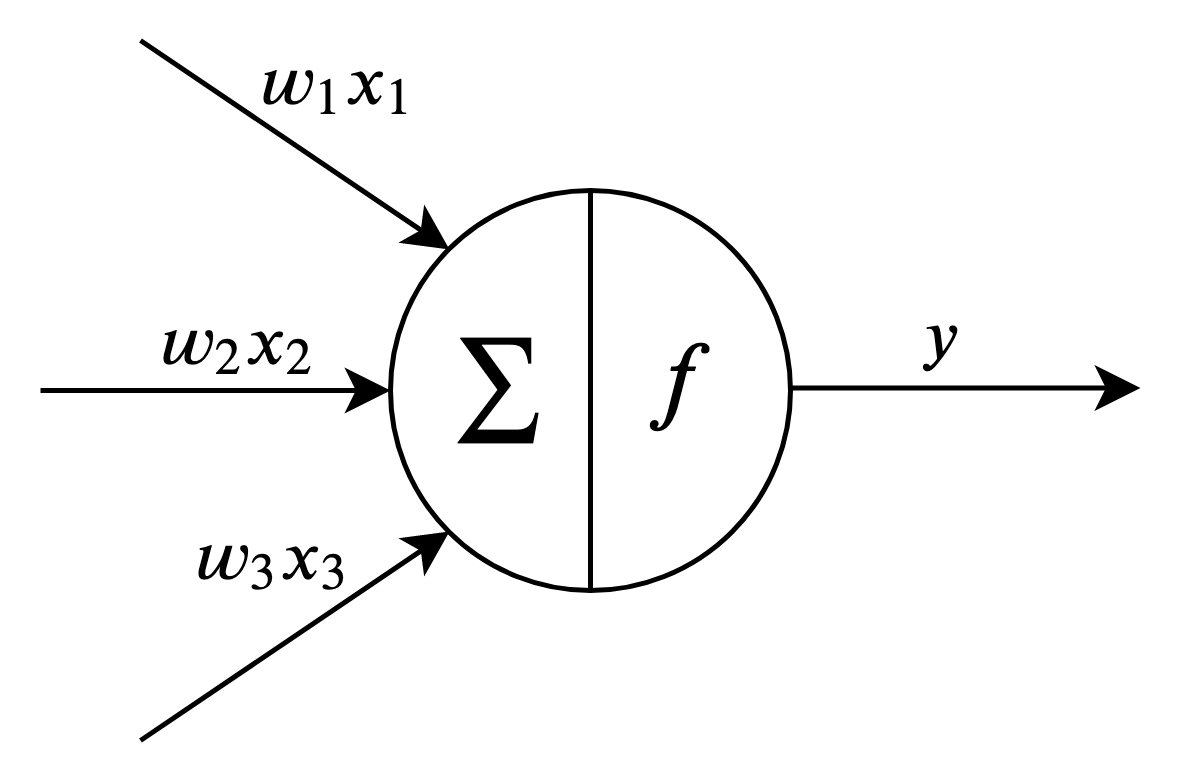
\includegraphics[width=2in]{figures/neuron}
	\caption{A neuron with 3 inputs; bias term omitted for simplicity.}\label{neuron}
\end{figure}


\subsection{Fully-Connected Layers}
A fully-connected layer is a vector of neurons. All neurons in a fully-connected layer receive the same input vector. This vector is the previous layer's output. A fully-connected layer with 3 neurons receiving input from an input layer is shown in figure \ref{fully-connected}. The output is a vector comprising of the outputs of each neuron. Each neuron output is calculated using the $M$-sized input vector as shown in equation \label{n-act} and added to output vector $\mathbf{y}$.
\begin{align}
y_i &= f_{\text{act}}\left( b + \sum_{j=1}^{M}(w_jx_j) \right) \ref{n-act} \\
\mathbf{y} &= \left\{ y_1, y_2, \ldots, y_n \right\} 
\end{align}

\begin{figure}
	\centering
	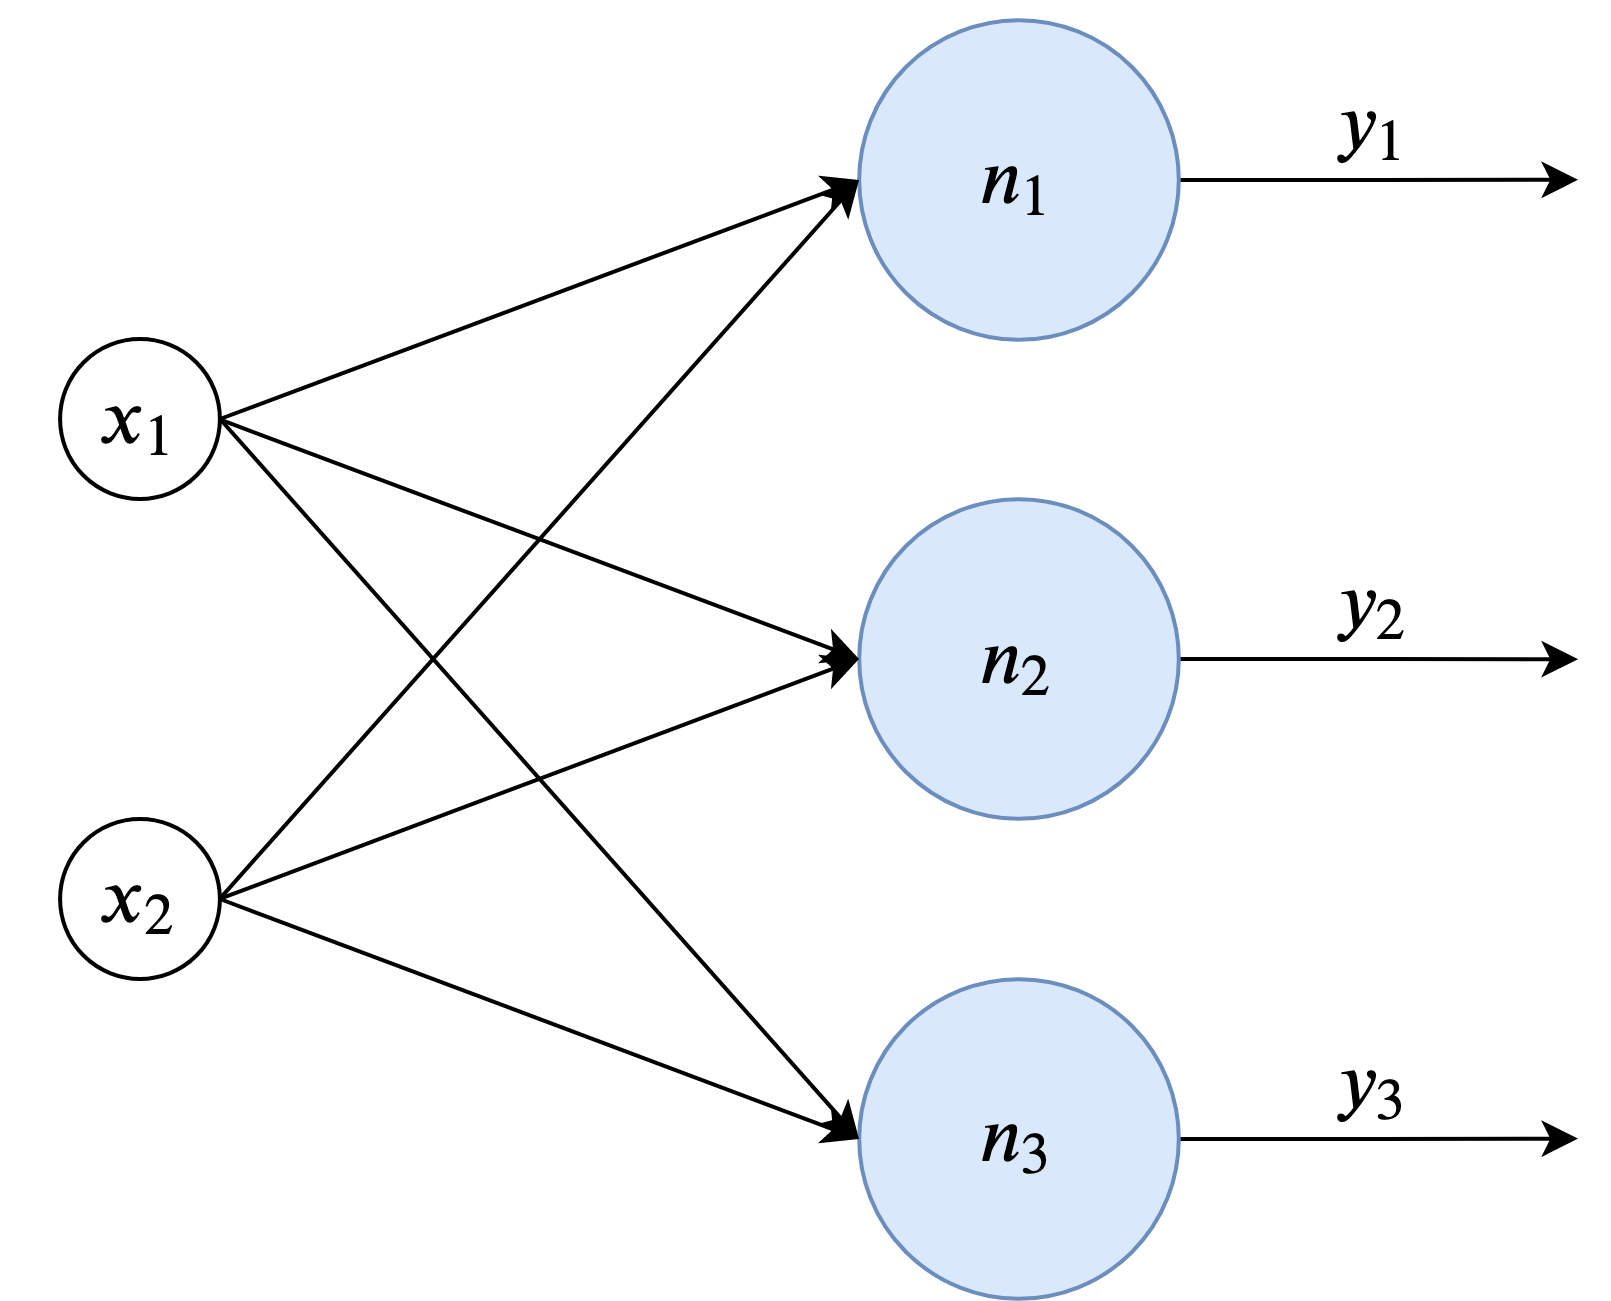
\includegraphics[width=3in]{figures/fully-connected}
	\caption{A fully-connected layer with 3 neurons, each receiving an input vector of size 2 from the input layer.}\label{fully-connected}
\end{figure}

\subsection{Activation Functions}
Without activation functions, the neural network would simply devolve to a linear classifier. Activation functions provide neural networks with the non-linearity to solve complex classification problems. Two of the most common activation functions are the rectified linear unit (ReLU) and the softmax function. These are the two activation functions that were chosen to be used in the software and hardware models of this thesis.

\paragraph{ReLU}
ReLU is a powerful activation function that has found widespread use due to its mathematical simplicity. The ReLU function is shown in equation \ref{relu-func}.
\begin{align}
y = \max(0, x) \label{relu-func}
\end{align}
Notably, the ReLU function is much easier to compute compare to the sigmoid or hyperbolic tangent functions, which both use the exponential function. The ReLU function also quite frequently performs just as well if not better compared to other activation functions. One of the reasons is because it does not suffer as much from the vanishing gradient problem \cite{pmlr-v15-glorot11a}. The vanishing gradient problem is encountered during training using backpropagation, which is covered briefly in section \ref{backprop}. As the gradients are generally small and since the chian rule Since ReLU only saturates in one direction, ReLU networks will be more sparse, in the sense that many of the neurons will have an output of 0. 

\paragraph{Softmax}


\subsection{Cross-Entropy Loss}

\subsection{The Backpropagation Algorithm}\label{backprop}


\section{Related Work}